%
% defintion.tex -- MSA definition
%
% (c) 2019 Prof Dr Andreas Müller
%
\section{Skalen und Vektorräume
\label{section:skalen und vektorraeume}}
\rhead{Skalen und Vektorräume}

\subsection{Ein Turm von Vektorräumen}
Wir möchten zum Ausdruck bringen, dass Funktionen in $L^2(\mathbb R)$
mit zunehmender Genauigkeit approximiert werden können durch Funktionen,
die immer mehr Einzelheiten auflösen.
Sei also $V_0\subset L^2(\mathbb R)$ eine Menge von Funktionen, wobei wir
uns vorstellen, dass darin Funktionsdetails bis zur Länge eins aufgelöst
sind.
Im Beispiel des Haar-Wavelets wäre der Raum der Funktionen, die
zwischen ganzzahligen $t$-Werten konstant sind, ein geeigneter Raum,
der diese Intuition wiedergibt.

Wir erwarten, dass $V_0$ dazu geeignet ist, Funktionen aus $L^2$ auf
eine translationsinvariante Art zu approximieren.
Das geht aber nur, wenn mit $f\in V_0$ auch alle verschobenen Funktionen
$T_bf\in V_0$ sind für $b\in\mathbb Z$.

Durch Skalierung von Funktionen wird es möglich werden, weitere Details
aufzulösen.
Der Vektorraum $V_j$ soll die Menge der Funktionen umfassen, die Details
bis zur Grösse $2^{-j}$ darstellen kann.
Im Haar-Wavelet-Beispiel sind das die Funktionen, die zwischen Punkten
konstant sind, die ganzzahlige Vielfache von $2^{-j}$ sind.
Je mehr Details aufgelöst werden können, desto grösser sind die
Vektorräume.
Es entsteht ein Turm
\begin{equation}
\dots
V_{-2}\subset
V_{-1}\subset
V_0\subset
V_1\subset
V_2\subset
\dots
V_j\subset
\dots
\subset L^2(\mathbb R)
\label{buch:skalen-turm}
\end{equation}
von Unterräumen von $L^2(\mathbb R)$.

Der Turm~\eqref{buch:skalen-turm} drückt noch nicht aus, dass die
Funktionen, die höhere Details wiedergeben, skalierte Versionen der
``gröberen'' Funktionen sind.
Daher wird gefordert, dass
\[
f\in V_j \quad\Rightarrow\quad D_2f\in V_{j+1}
\qquad\text{oder}\qquad
D_2V_j \subset V_{j+1}
\]
Dies drückt aber noch nicht aus, dass in $V_{j+1}$ noch mehr Details
aufgelöst werden können, als mit Hilfe von skalierten Versionen der
Funktionen in $V_j$ möglich ist.
Dazu muss verlangt werden, dass
$D_2V_j = V_{j+1}$
gilt.

Es wäre zu viel verlangt, dass jede Funktion in $L^2(\mathbb R)$ in
einem der Vektorräume $V_j$ liegt, denn in $L^2(\mathbb R)$ gibt
es ja einige ``ganz verrückte'' Funktionen.
Die Abtastung soll also detailliert genug sein, dass jede 
Funktion in $L^2(\mathbb R)$ beliebig genau durch Funktionen aus
der Vereinigung aller $V_j$ approximiert werden kann.
Dies wird durch
\[
\overline{\bigcup_{j\in Z} V_j} = L^2(\mathbb R)
\]
ausgedrückt, wobei der Querstrich den Abschluss, die Menge aller Grenzwerte
von Folgen der Vereinigung der $V_j$ bezeichnet.

Wird die Auflösung schrittweise reduziert, dann bleibt nur die Nullfunktion
übrig.
Es gibt also keine Funktionen mit Features, die beliebig weit ausgedehnt
sind im Sinne der Vektorräume $V_j$.
Man kann dies durch
\[
\bigcap_{j\in\mathbb Z} V_j = \{0\}
\]
ausdrücken.

Damit haben wir alle Elemente zusammen für die formale Definition.

\begin{definition}
Eine {\em Multiskalen-Analyse} ist ein Turm
\[
\dots
V_{-2}\subset
V_{-1}\subset
V_0\subset
V_1\subset
V_2\subset
\dots
V_j\subset
\dots
\]
von Unterräumen von $L^2(\mathbb R)$
mit den folgenden Eigenschaften
\begin{enumerate}
\item Es gibt eine Funktion $\varphi\in V_0$ derart, dass die Funktionen
$T_k\varphi$ eine orthonormierte Basis von $V_0$ bilden.
\item $D_{\frac12} V_j = V_{j+1}$
\item $\bigcap_{j\in\mathbb Z} V_j = \{0\}$
\item $\overline{\bigcup_{j\in\mathbb Z} V_j} = L^2(\mathbb R)$.
\item Es gibt eine Funktion $\psi\in V_0$ derart, dass
die Translate $T_b\psi$ mit $b\in\mathbb Z$ den Raum $W_0$ erzeugen:
\[
W_0 = \overline{\langle T_b\psi\;|\;b\in\mathbb Z\rangle}.
\]
\end{enumerate}
\end{definition}

\begin{figure}
\centering
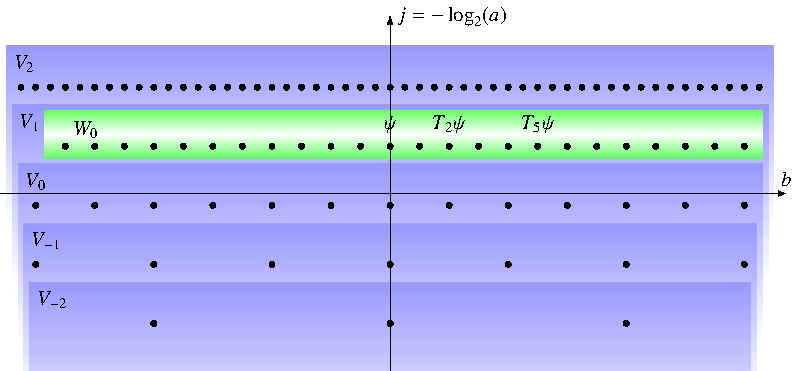
\includegraphics{chapters/6-msa/images/msa.pdf}
\caption{Hierarchie der Vektorräume $V_j$ sowie der Komplemente $W_j$
mit
$V_{j+1} = V_j \oplus = W_j$.
\label{msa:vektorraumhierarchie}}
\end{figure}

Man beachte, es wird nicht verlangt, dass die $T_b\psi$ orthogonal
sein müssen.

\begin{beispiel}
Das Haar-Wavelet erzeugt eine Multiskalen-Analyse von $L^2(\mathbb R)$.
% XXX TODO Haar MRA darstellen
\end{beispiel}

\begin{beispiel}
% XXX TODO MRA der auf 2-adischen Intervallen stückweise linearen Funktionen
\end{beispiel}

\subsection{Orthogonalität}

% XXX TODO Kette von Vektorräumen
% XXX TODO V_j und W_j
% XXX TODO Orthogonalitätseigenschaften
% XXX TODO Projektionsoperatoren
